\chapter{Introdução}

O mundo está envelhecendo de forma cada vez mais rápida. De acordo com as 
estimativas da Organização das Nações Unidas (ONU), há uma tendência não só 
ao crescimento populacional em geral, mas um crescimento da população acima de 60 anos, 
que deve triplicar nos próximos 40 anos. Com o aumento da população idosa há também 
o aumento de pessoas com mobilidade reduzida, e assim, cada vez mais torna-se 
necessário o uso de sistemas que auxiliem na movimentação e também no monitoramento 
das atividades destes.\\

Segundo levantamento em relatório da Organização Mundial da Saúde (OMS), 
anualmente, cerca de 500 mil pessoas no mundo ficam incapacitadas devido a 
lesões medulares. Com esses altos índices, existe outro fator de aumento 
nos índices de pessoas com mobilidade reduzida, e com isso, a necessidade 
de alternativas que melhorem cada vez mais a qualidade de vida e aumentem a 
independência destes pacientes.\\

Apesar da existência de diversos modelos de cadeiras de rodas motorizadas, 
o alto custo de sua grande maioria torna a aquisição inviável para pessoas de 
baixa renda. 
Com preços oscilando até cerca de R\$ 20.000,00, grande parte da população de 
usuários continua a optar por modelos mais simples e sem motorização, aumentando a 
dependência do usuário de um cuidador presente a todos os momentos.\\

\section{O Problema}

O desenvolvimento da opção mais básica de mobilidade para portadores de mobilidade
reduzida, a cadeira de rodas, vem tornando-se cada vez mais estagnada. 
Mesmo com a adaptação do modelo clássico para modelos motorizados, não há, 
fora isso, muitas outras opções de mercado a fim de valorizar o conforto 
e facilitar a vida do usuário e seus familiares. Atualmente, a oferta de 
cadeira de rodas motorizadas com tecnologias semelhantes torna-se cada 
vez mais comum em um cenário onde um alto número de pessoas continua a optar 
por modelos clássicos devido aos altos custos dos modelos presentes no 
mercado internacional. A falta de opções com novas funcionalidades no mercado 
e o alto custo das soluções já existentes tornam o acesso a essas novidades
 cada vez mais restrito.\\
	
Além disso, a ausência de um familiar ou cuidador em certos momentos 
do dia 
dificulta o monitoramento de atividades motoras ou necessidades 
do usuário. 
Com isso em foco, o monitoramento remoto contínuo do usuário 
poderia 
aumentar ainda mais sua liberdade em um ambiente doméstico e, ainda 
assim, 
manter familiares e cuidadores atentos a sinais e alertas e evitando 
possíveis 
acidentes e situações fora do cotidiano.\\
	
O problema, juntamente às suas causas, são representados em um diagrama 
de Causa e Efeito, ou fishbone, conforme Figura \ref{fishbone}.
	
\begin{figure}[h]
    \centering
    \label{fishbone}
    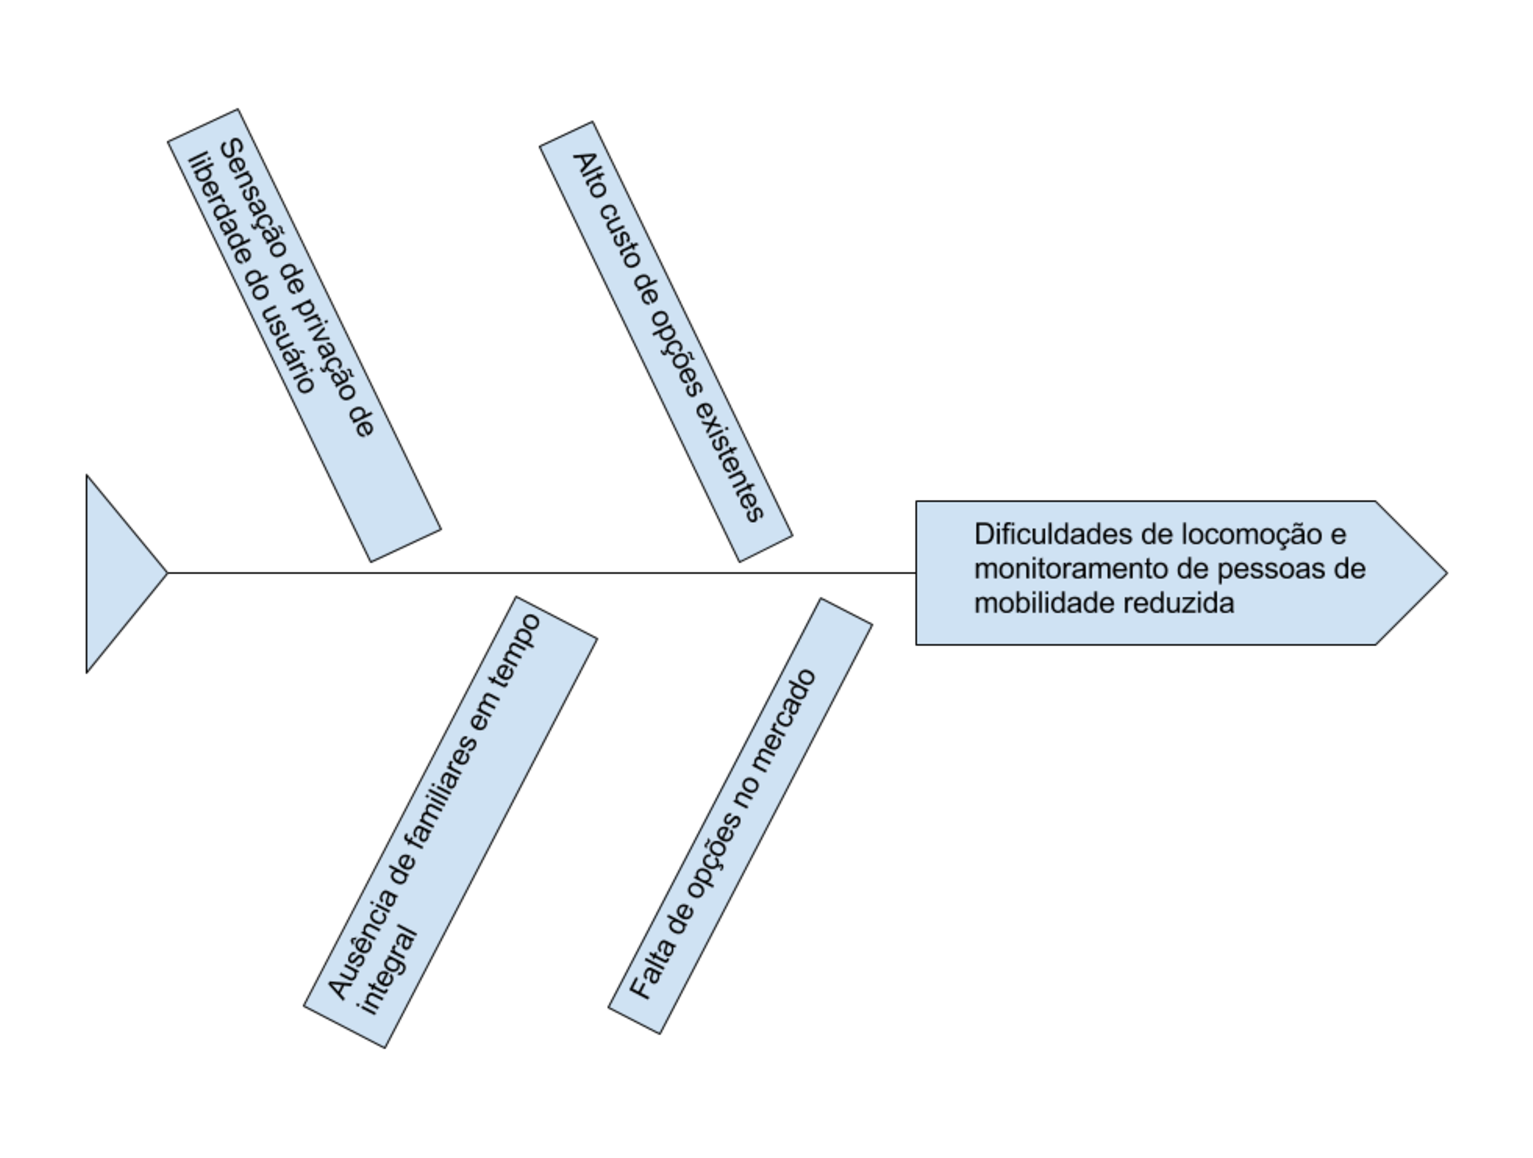
\includegraphics[keepaspectratio=true,scale=0.5]{figuras/fishbone.eps}
    \caption{Diagrama de causa e efeito (\textit{fishbone}) para mapeamento do problema.}
\end{figure}


\section{Estado da Arte}

Dentre as opções para cadeiras de rodas motorizadas acessíveis existentes no mercado,
é comum deparar-se com alternativas para adaptação de cadeiras convencionais,
como por exemplo o sistema \textit{Light Drive} produzido pela empresa britânica, 
com sede em Bristol, \textit{Benoit Solutions}. Este sistema consiste em um \textit{kit}
contendo um baterias, dois motores, uma roda traseira para prevenção de possíveis
acidentes e quedas, e um sistema de controle do tipo \textit{joystick}
para controle de velocidade e direção da cadeira de rodas.\\

Na Figura \ref{ldrive} é possível visualizar os componentes do sistema e
o sistema inserido em uma cadeira de rodas convencional.

\begin{figure}[h]
    \centering
    \label{ldrive}
    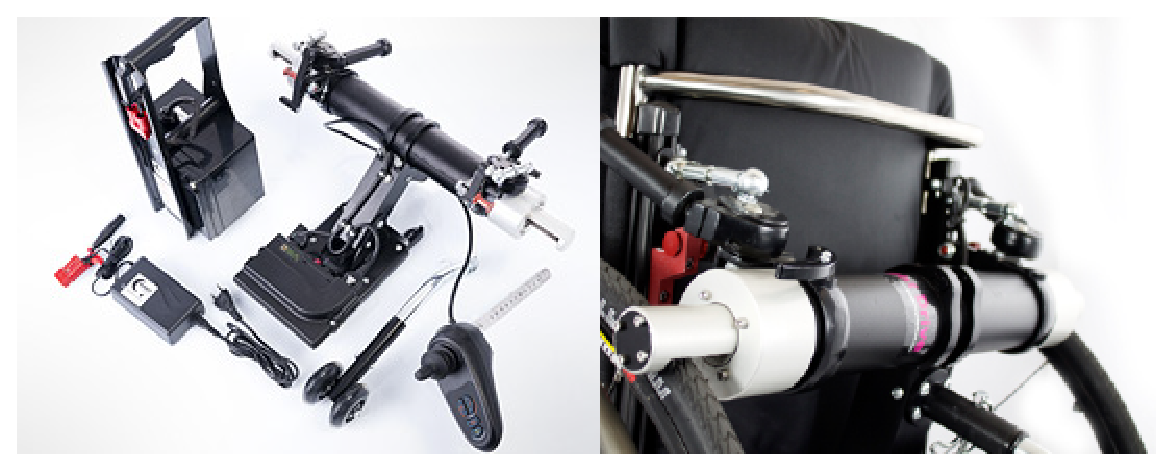
\includegraphics[keepaspectratio=true,scale=0.7]{figuras/ldrive.eps}
    \caption{Sistema de adaptação \textit{Light Drive} da empresa britânica \textit{Benoit Solutions}.}
\end{figure}

O sistema utiliza dois motores de 12V e 100W de potência para a movimentação 
de cadeiras de rodas convencionais, que geralmente possuem pesos de cerca de 16Kg 
e possui um sistema de baterias que pode ser escolhido pelo usuário entre modelos 
de Níquel Metal Hidreto  (NiMH) ou Chumbo-Ácido, ambas com capacidades de 10Ah 
e controle de movimentação e velocidade via \textit{joystick} localizado no 
suporte para braços da cadeira de rodas.\\

No que tange soluções para cadeiras de rodas convencionais ou motorizadas
com sistemas de monitoramento, não há alternativas presentes no mercado
atual, tornando o projeto UMISS um novo produto a ser inserido no contexto
de sistemas de monitoramento e locomoção, definindo o mesmo como estado da arte.

\section{Objetivos}
Esta seção possui as especificações dos objetivos do projeto a ser desenvolvido.

\subsection{Geral}
O projeto possui como objetivo a contrução de uma cadeira de rodas motorizada capaz de
oferecer capacidade de locomoção para pessoas com mobilidade reduzida
e, que possa realizar
a aquisição e processamento de sinais vitais do usuário para fins de alerta e notificação
remota de terceiros.

\subsection{Específicos}

\begin{itemize}
\item Dimensionar e contruir uma estrutura da cadeira de rodas;
\item Identificar e selecionar melhor técnica para aquisição e condicionamento de sinais provenientes do usuário;
\item Desenvolver sistema embarcado capaz de processar e transmitir dados capturados;
\item Desenvolver plataforma para apresentação de dados e alertas;
\item Dimensionar e desenvolver sistemas de movimentação e controle da cadeira de rodas;
\item Dimensionar sistema de alimentação;
\end{itemize}

\section{Proposta de Solução}

Fazer uma proposta de sistema EM ALTO NÍVEL sobre o problema, e porque essa solução é melhor que as mencionadas na seção anterior.

\section{Escopo}

O que a solução deverá abranger e não abranger.


\section{Termo de Abertura do Projeto}
Este documento tem como objetivo a formalização do projeto Unidade Móvel de
Identificação de Saúde e Socorro (UMISS). As informações contidas nos tópicos 
a seguir foram produzidos a fim de mostrar um resumo dos objetivos, riscos, 
limites e recursos, bem como mostrar o estudo de viabilidade do projeto. 
Tendo em vista as limitações de prazo, dinheiro e infraestrutura dos 
participantes do projeto.
\subsection{Descrição do Projeto}
Para ter uma visão clara do projeto, foi usado o mapeamento de atividade no 
modelo 5W2H, que está descrito a seguir:

\begin{itemize}
    \item \textbf{What:} Sitema integrado com subsistemas de movimentação,
    monitoramento e estrutura. Desenvolvendo uma cadeira com possibilidade
    de movimentação e captação dos sinais enviados pelo paciente. E monitoramento
    através de um aplicativo nativo android e de uma plataforma web.
    \item \textbf{Why:} Movimentar um indivíduo com mobilidade reduzida
    e enviar respostas recolhidas
    dos sensores para aplicativos e plataformas web dos seus respectivos
    cuidadores.
    \item \textbf{Where:} Em qualquer ambiente que tenha acesso a uma rede wifi.
    \item \textbf{When:} Durante o primeiro semestre de 2017.
    \item \textbf{Who:} Alunos dos cursos de Engenharias do Campus UnB Gama, nos
    quais estão cursando a matéria de Projeto Integrador 2.
    \item \textbf{How:} Utilizando a orientação dos professores da Universidade
    de Brasília.
    \item \textbf{How Much:} Cerca de R\$ 3.000,00, quanto a equipamento, por
    cadeira.
\end{itemize}

\subsection{Propósito e justificativa do Projeto}
O projeto tem como objetivo oferecer à pessoas indivíduo com mobilidade reduzida
e seus cuidadores,
a um preço acessível, uma cadeira de rodas motorizada, com fácil dirigibilidade 
e que tenha total controle sobre os sinais vitais do paciente, a fim de avaliar 
as condições do mesmo e julgar se ele está em estado normal de saúde ou corre 
algum risco. Neste caso, os cuidadores, que poderiam ser parentes, amigos 
próximos e médicos ou enfermeiros contratados, seriam notificados, com atraso 
um mínimo, do seu estado através de um site e um aplicativo.

O desenvolvimento do produto se justifica uma vez que as cadeiras motorizadas 
são muito caras no mercado atual, além de que não existe nenhuma que possui 
um sistema de monitoramento da saúde do paciente, dificultando, então, seu 
resgate caso alguma emergência se faça presente. O que facilita em termos de 
preocupação e tempo, a vida dos cuidadores, uma vez que não será mais necessária
a presença contínua ao lado do paciente, já que a cadeira fará esse papel.

\subsection{Restrições do Projeto}
As restruções do projeto UMISS são as descritas as seguir:
\begin{itemize}
    \item Limite de integrantes de acordo com os percentuais de inscritos na disciplina no semestre do trabalho;
    \item Limitação de custos do projeto, calibrado pela quantidade que o grupo estará disposta a colaborar;
    \item O projeto está restrito ao tempo da disciplina de Projeto Integrador
   2 (06/03/2017 - 29/06/2017).
    \item Estar de acordo com as exigências do cliente, composto pelos Docentes
    da Universidade de Brasília da Unidade Gama.
\end{itemize}

\subsection{Riscos do Projeto}
Os principais riscos presentes na execução do Projeto UMISS, bem como suas medidas preventivas, estão explícitas a seguir:

\begin{itemize}
    \item Falta de experiência dos membros dos projetos nos deveres de cada 
    subárea

Plano de ação: Cada subárea irá mapear e corrigir possíveis lacunas de 
conhecimento para a realização das tarefas

    \item Membro da equipe trancar ou abandonar a disciplina.

Plano de ação: Distribuir as tarefas entre os integrantes remanescentes de 
forma que não sobrecarregue nenhum dos membros da equipe.

    \item Falta de horário comum entre os membros

Plano de ação: Combinar encontros online e presenciais por meio das mídias de 
comunicação em horário não comercial.

    \item Falta de experiência em gerência de projeto

Plano de ação: Obter feedbacks dos membros sobre a atuação e gerar planos de 
ação para melhorar cada ponto levantado.

    \item Possível descompromisso de membros da equipe

        Plano de ação: Realizar reuniões com o membro oferecendo suporte nas dificuldades levantadas

    \item Não cumprimento do cronograma sugerido

        Plano de ação: Ajustas datas de cronograma de forma a acelerar prazos atrasados

    \item Alteração de requisitos de projeto

        Plano de ação: Repensar o escopo do projeto afim de adapá-lo aos novos requisitos

    \item Queima ou danos em componentes do projeto

        Plano de ação: Compra de novos componentes ou recondicionamento de itens danificados

    \item Atraso na entrega de pedidos para o projeto

        Plano de ação: Procurar fornecedores locais para os componentes ou contratar frete expresso para entrega.
\end{itemize}



\subsection{Custos do Projeto}
De acordo com o \ref{relatoriogestao} da UnB o custo médio por aluno 
anual é de R\$12.100,00.

Considerando que o curso de Engenharia, no qual os alunos das 
disciplinas estão matriculados, exige 240 créditos para um aluno se formar em 
5 anos(10 semestres) e que cada crédito corresponde à 15 
horas/aula. Sendo assim o custo de formar um aluno na UnB é de 5 
vezes o custo anual(R\$12.100,00),ou seja, R\$60.500,00.

Diante disso, é possível concluir que se multiplicarmos 240(créditos) por 
15(horas/aula) obtemos o valor total de horas para se formar um aluno da UnB,
sendo esse valor total de 3.600 horas. Se dividirmos o custo total de 
formação(R\$60.500,00) pelo total de horas(3.600) teremos o custo da hora 
de um aluno da UnB, sendo esse valor R\$16,80 (reais/hora).

O projeto ocorrerá em um período de 15 semanas durante um semestre com data 
final a apresentação do segundo ponto de controle 2 Release, projeto que no qual cada estudante irá 
dedicar 10 horas por semana a disciplina, ou seja, haverá um esforço de 150 
horas para a disciplina durante o semestre.

Deste modo cada aluno irá custar R\$2.520 ao projeto, visto que R\$2.520,00 é o 
resultado da multiplicação de 150 (horas) e de R\$16,80 (reais/hora).

Sendo que a equipe é composta por 13 integrantes(Equipe),estudantes de 
engenharia de software. Sendo assim se multiplicarmos os 10 integrantes pelo 
custo de cada integrante, teremos o custo total do projeto, que é de 
R\$32.760,00.

\subsection{Stakeholders}

\subsubsection{Cliente}
Hospitais e clinicas que lidam com pessoas de mobilidade reduzida. Usuários e financiadores do usuário.

\subsubsection{Equipe de Gerência}
Membros do projeto que tem a responsabilidade de planejamento, monitoramento 
e controle do projeto, garantindo a excelência e o sucesso do produto. Além 
disso tem a responsabilidade de tomar decisões fundamentais dentro do projeto, 
sendo eles:

\begin{table}[]
\centering
\caption{Equipe de Gerentes}
\label{equipe_gerentes}
\begin{tabular}{|l|l|}
\hline
Posição              & Indivíduo      \\ \hline
Gerente geral        & Afonso Delgado \\ \hline
Gerente de qualidade & Dylan Guedes   \\ \hline
Gerente de produto   & Rafael Amado   \\ \hline
\end{tabular}
\end{table}

\subsubsection{Equipe de Desenvolvimento}
Membros do projeto que tem a responsabilidade de construir o produto e a 
documentação necessária para a finalização do produto. Sendo eles: Mariana 
Andrade, Lunara Alves, César Antônio, Johnson Andrade, Felipe Costa, Lucas 
Matheus, Gustavo Cavalcante, Wilton da Silva, Tiago Ribeiro e Nivaldo Lopo.


\subsubsection{Docentes}
Professores da matéria Projeto Integrador 2 do primeiro semestre de 2017 que 
tem como responsabilidade avaliar o andamento e finalização do projeto e seu 
produto final. Sendo eles: Alex Reis, Sebastien Rondineau, Rhander Viana e 
Luiz Laranjeira.

\subsection{Produto do Projeto}
As entregas do produto serão feitas em três partes, dividos em pontos de controle

\textbf{Ponto de controle 01}: Definição do escopo e projeto, bem como o 
alinhamento. Concepção e detalhamento da solução.

\textbf{Ponto de controle 02}: Projeto e desenvolvimento de subsistemas.


\textbf{Ponto de controle 03}: Integração de subsistemas e finalização do 
produto.


